\documentclass[conference]{IEEEtran}
\IEEEoverridecommandlockouts
% The preceding line is only needed to identify funding in the first footnote. If that is unneeded, please comment it out.
\usepackage{cite}
\usepackage{amsmath,amssymb,amsfonts}
\usepackage{algorithmic}
\usepackage{graphicx}
\usepackage{fontspec}
\usepackage{caption}
\usepackage{subcaption}
\usepackage{array}
\newcommand\tab[1][1cm]{\hspace*{#1}}
\usepackage{hyperref}
\hypersetup{
    colorlinks=true,
    linkcolor=blue,
    filecolor=magenta,      
    urlcolor=cyan,
}

%for typing Myanmar text, you can also used with Myanmar3 font
\newfontfamily {\padauktext}[Script=Myanmar]{Padauk}
%\newfontinstance {\padauktext}[Script=Myanmar]{Padauk}

%for double quote
\newcommand{\quotes}[1]{``#1''}

%\def\BibTeX{{\rm B\kern-.05em{\sc i\kern-.025em b}\kern-.08em
 %   T\kern-.1667em\lower.7ex\hbox{E}\kern-.125emX}}

%\def\baselinestretch{0.94}

\begin{document}

\title{Automatic Speech Recognition System for Burmese Sentences using Kaldi\\
%{\footnotesize \textsuperscript{*}Note: Sub-titles are not captured in Xplore and %should not be used}
%\thanks{Identify applicable funding agency here. If none, delete this.}
}




\author{
\IEEEauthorblockN{Hlaing Myat Nwe}
\IEEEauthorblockA{\textit{hlaingmyatnwe@utycc.edu.mm} }
\and
\IEEEauthorblockN{Khant Khant Win Tint}
\IEEEauthorblockA{\textit{khantkhantwintint@utycc.edu.mm} }
\and
\IEEEauthorblockN{Khaing Hsu Wai}
\IEEEauthorblockA{\textit{khainghsuwai@utycc.edu.mm} }
}


\maketitle

\begin{abstract}
The accuracy of automatic speech recognition (ASR) remains one of the most important research challenges based on the vocabulary size, noise and the variety of language and speaker. This project is aimed to built an accurate automatic speech recognition system for small amount of data-set using Kaldi, an open-source toolkit for speech recognition written in C++. In this project, we made three types of experiment. First of all, we applied the incremental training concept and different approaches of training and adaptation techniques are studied in order to improve the recognition accuracy. Second, we used different n-gram language models to investigate the accuracy and evaluated the performance of the model depending on the different model size. For training the acoustic part of the model, Hidden Markov Model and Gaussian Mixture Model is used. The performance of the system is evaluated in terms of Word Error Rate (WER).
\end{abstract}

\begin{IEEEkeywords}
Automatic Speech Recognition, Acoustic Model, Kaldi, Hidden Markov Model, Gaussian Mixture Model
\end{IEEEkeywords}

\section{Introduction}
\label{sec:intro}

Speech is the general communication language for humans. In speech processing, automatic speech recognition (ASR) is a process that converts human speech to a sequence of words which is spoken by human. The use of speech for interacting with the computer may assist the developing country as the language technologies being implemented for the e-governance system. There is only a few of works have been done in ASR for Myanmar language. The major difficulty in the research process of Myanmar language ASR is the lack of Myanmar speech corpus. Generally, it is not easy to build the speech corpus because it requires a huge amount of speech data, time, and efforts.

The main problem of the ASR is the complexity of the human language. In speech recognition system, many parameters may also affect the performance of recognition such as the vocabulary size, noise and the variety of language and speaker. In this project, different approaches have been tried to get good performance of the speech using different parameters.

The main purpose of this project is to develop more efficient acoustic model that is one of the main components of the ASR to get the better accuracy of small Myanmar ASR model. Better accuracy can be achieved if the efficient acoustic modeling approach is applied. In this project, Gaussian Mixture Model-Hidden Markov Model (GMM-HMM) based acoustic model is built for developing the Myanmar ASR using Mel Frequency Cepstral Coefficient (MFCC) feature extraction technique. The hyperparameters of GMM-HMM are optimized to improve the ASR performance for Myanmar language. In this work, we used SRILM to build language model for Myanmar language and weighted finite-state transducers for decoding ASR. In our experiment, we made three types of evaluation based on the amount of training data, language model and number of model size in terms of WER\%. We also applied and compared different approaches of training and adaptation techniques. Furthermore, We have applied myG2P mapping to create a lexicon file ~\cite{YKTG2P}.

Among many toolkits for the implementation of speech recognition, we used Kaldi toolkit, an open-source toolkit made for dealing with speech data in our project. It is written in C++ and licensed under the Apache License v2.0 ~\cite{howtostartKaldi}. 

\section{Data Preparation}
\label{sec:DataPreparation}
Data preparation is a necessary step to set up ASR system with our own data. There are three parts to prepare: audio data, acoustic data and language data. 

\subsection {Audio Data}
\label{subsec:AudioData}
Firstly, we prepared audio data to set up an ASR system based on that data. We recorded the audio files with the students of NLP class in the E-learning studio room of University of Technology (Yatanarpon Cyber City). File format that we used is WAV. The set parameters of audio are mono channel, 16kHz sampling frequency rate and the record second is 3. Each file contains one short sentence. Each of these audio files is named in a recognizable way and placed in the recognizable folder representing particular speaker. 
In this project, we prepared four types of dataset for the incremental training such as we used 6 speakers for first experiment, 10 speakers for second experiment, 16 speakers for third experiment and 20 speakers for fourth experiment. The audio dataset used for our experiment is described as shown in Table~\ref{table:audioData}.

\begin{table}[ht]
\caption{Data used for Incremental Training} % title of Table
\centering % used for centering table
\setlength\tabcolsep{1.5pt} % default value: 6pt
\begin{tabular}{c c c c} % centered columns (4 columns)
\hline %inserts double horizontal lines
Experiment & No. of & No. of Sentences & No. of Sentences \\  %[0.5ex] % inserts table
%heading
  & Sentences & for Training & for Testing  \\
\hline % inserts single horizontal line


1st Experiment &  6 & 2100 & 900\\
2nd Experiment &  10 & 3500 & 1500\\
3rd Experiment &  16 & 5600 & 2400\\ % inserting body of the table
4th Experiment &  20 & 7000 & 3000\\[1ex] % [1ex] adds vertical space
\hline %inserts single line
\end{tabular}
\label{table:audioData} % is used to refer this table in the text
\end{table}


\subsection {Acoustic Data}
\label{subsec:AcousticData}
We created some text files to communicate with our audio data. In this project, we collected 500 general sentences for each speaker. Example sentences can be seen in Figure~\ref{fig:acdatafig}. We prepared text files that relates to the specific recordings:

\subsubsection{text}
\label{subsec:text}
It contains the information about every utterance ID matched with its text transcription.

\subsubsection{spk2gender}
\label{subsec:spk2gender}
It informs about speakers gender.

\subsubsection{utt2spk}
\label{subsec:utt2spk}
It tells the ASR system which utterance belongs to particular speaker.

\subsubsection{wav.scp}
\label{subsec:wav.scp}
It connects every utterance (sentence said by one person during particular recording session) with an audio file related to this utterance.

\begin{figure}[htbp]
\centerline{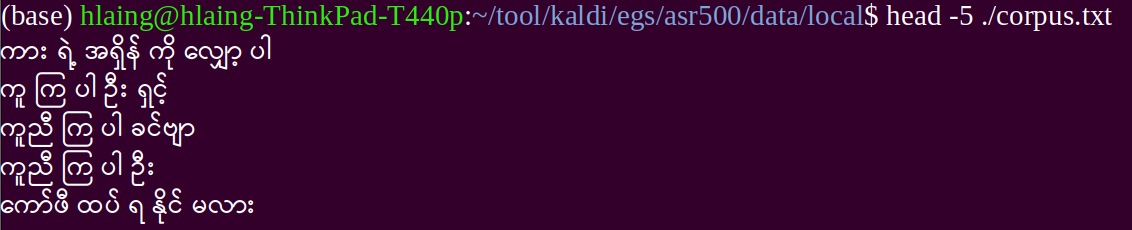
\includegraphics[width=3.5in, height=0.7in]{acdata.png}}
\caption{Example Sentences that used in this project}
\label{fig:acdatafig}
\end{figure}

\subsection{Language Data}
\label{sec:LanguageData}
Grapheme-to-Phoneme (G2P) conversion is about predicting the pronunciation of words given only the spelling. Grapheme-to-Phoneme (G2P) conversion models are also very important for natural language processing (NLP), automatic speech recognition (ASR) and text-to-speech (TTS) developments. For our experiment, we applied myG2P models to create lexicon file. Lexicon file that contains every word from dictionary with its phone transcription is vital for improving the ASR accuracy. It was as shown in Figure~\ref{fig:ldatafig}. Moreover, we also collected and prepared some text files for silence, nonsilence and optional silence phones of our corpus. 
\begin{figure}[htbp]
\centerline{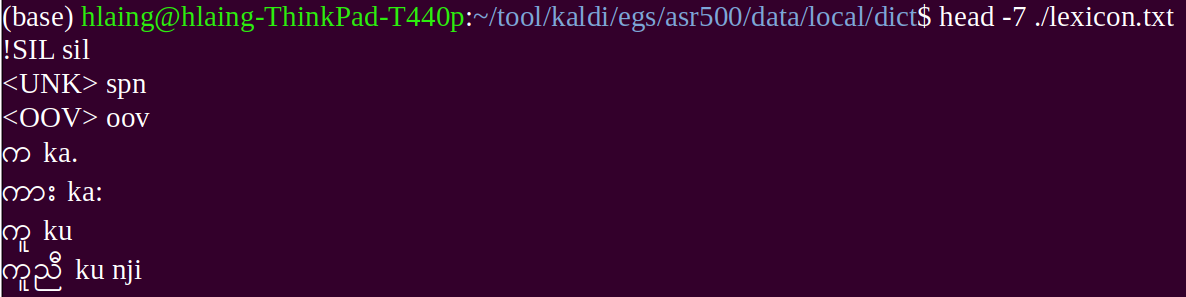
\includegraphics[width=3.5in, height=0.7in]{Fig2.png}}
\caption{Example of Myanmar Lexicon}
\label{fig:ldatafig}
\end{figure}


\section{Methodology}
\label{sec:Methodology}
In this section, we describe the methodology used in our experiments.

\subsection{Feature Extraction}
\label{subsec:FeatureExtraction}
Feature extraction is an essential first step in speech recognition applications. The goal of the feature extraction is to extract sequences of acoustic observations that contain all the useful features and information for recognition operation. There are several methods used in the feature extraction operation, such as Mel frequency cepstral coefficients (MFCC), Feature space transformations, perceptual linear prediction (PLP), Cepstral mean and variance normalization (CMVN), Kernal Based Feature Extraction, and Dynamic Feature Extraction. In this project, we are going to make use of MFCC was used with the aim of reducing the spectral distortion by shrinking the beginning and end of each frame of the signal to zero ~\cite{gmm}. These are based on the main idea of the cepstrum.

In addition, static features were extracted from each frame of speech data and it is beneficial to use some transformations to improve the recognition. There are transforms, projections and other feature operations: Frame splicing and Delta feature computation, Linear Discriminant Analysis (LDA) transform, Heteroscedastic Linear Discriminant Analysis (HLDA) and Maximum Likelihood Linear Transform (MLLT) estimation [4]. We used and compared both Delta feature computation and LDA+MLLT.

\subsubsection{Delta feature computation}
\label{subsec:Deltafeaturecomputation.}
MFCC feature only takes account of the relationship in phonetic frames without considering the relationship between them. Delta feature is the Fourier Transform of the time order of the phonetic frames order. For instance: If we have 13 MFCC coefficients, with the delta and double-delta (Δ+ΔΔ) transformation we also get 13+13 delta coefficients, which would combine to give a feature vector of length 39 (13+13+13). Then, the original vector is reduced to vector of 30 MFCC Δ+ΔΔ acoustic features.

\subsubsection{LDA+MLLT}
\label{subsec:LDAMLLT}
LDA is a linear transform that reduces dimensionality of our input features. The idea of LDA is to find a linear transformation of feature vectors from an n-dimensional space to vectors in an m-dimensional space (m<n) such that the class separability is maximum. MLLT estimates the parameters of a linear transform in order to maximize the likelihood of the training data given a diagonal-covariance Gaussian mixture models; the transformed features are better represented by the model than the original features. 

\subsection{Acoustic Model}
\label{AcousticModel} 
The acoustic model is a very important component of the recognition process. The main goal for the acoustic model is to enhance the speech recognition accuracy by specifying the modeling units and computing the likelihood of the acoustic features' components for the phonetic units that need to be recognized. Acoustic models are trained by taking audio recordings of speech, and their text transcriptions, and creating statistical representations of the sounds that make up each word ~\cite{stot}. In ASR systems, most of the acoustic model stage uses the Hidden Markov Model (HMM) with the Gaussian Mixture Model (GMM) to extract the acoustic features vectors.

\subsubsection{Hidden Markov Model (HMM)}
\label{HiddenMarkovModel} 
HMM is a popular choice in speech recognition, being able to model this uncertainty between acoustic features and corresponding transcription ~\cite{meKaldi}. HMM is a stochastic finite state automaton that models the variation in the acoustic signal via a two-stage stochastic process. The automaton is defined through a set of states with transitions connecting the states. The probability P($x_1^T$|$w_1^N$) is extended by an unobservable (hidden) variables representing the states as in the following equation (1).

P($x_1^T$|$w_1^N$)=Σ P($x_1^T$,$s_1^T$|$w_1^N$)	 \tab[3cm](1)


\subsubsection{Gaussian Mixture Model (GMM)}
\label{GaussianMixtureModel} 
Gaussian Mixture Model (GMM) is a parametric probability density function which is represented as a
weighted sum of Gaussian component densities. It is used as a parametric model of probability distribution of measuring features in biometric systems. The GMM as a statistical model for Fourier-spectrum-based speech features plays an important role in acoustic modeling of conventional speech recognition systems. GMM is used as a classifier to compare the features extracted from the MFCC with the stored templates. GMM is represented by its Gaussian distribution and each Gaussian distribution is calculated by its mean, variance and weight of the Gaussian distribution ~\cite{gmm}.

In this project, GMM is used for estimating the output distribution \{$b_j$()\}. Gaussian mixture models are able to describe such multimodality thus making GMMs a powerful tool in speech recognition. The expression for the output observation becomes as in (2).

$b_j$ (x) = Σ$^M_m_=_1$ $c_j_m$ N(x; \mu^j^m, $Σ^j^m$) \tab[1.5cm](2)

where $c_j_m$ is the prior probability for component m of state $s_j$ and N(x; \mu^j^m, $Σ^j^m$) is the Gaussian (or normal) disitribution with parameters \mu^j^m \& $Σ^j^m$ corresponding to the mean and covariance of state $s_j$ respectively. The prior probabilities satisfy the probability mass function constraints as in (3).

Σ$^M_m_=_1$ $c_j_m$=1, $c_j_m$>=0 \tab[3.5cm](3)

If M is set to equal one, a single Gaussian distribution is obtained. In the training of a GMM the aim is to update the mean and covariance: \mu^j^m , $Σ^j^m$ .

\subsection{Language Model}
\label{sec:LanguageModel}

The language model P( $w_1^N$ )provides a prior probability for the word sequence $w_1^N$ = w1,..., wN. Thus, it inherently aims at capturing the syntax, semantics, and pragmatics of a language. Since language models are independent of acoustic observations, their parameters can be estimated from large text collections. Due to a theoretically infinite number of possible word sequences, language models require suitable model assumptions to make the estimation problem practicable. For large vocabulary speech recognition, n-gram language models have become widely accepted. An n-gram language model is based on the assumption that a sequence of words follows an (n-1)-th order Markov process, that is, the probability of a word wn is supposed to depend only on wn-1 predecessor words ~\cite{acmdl} as in (4).

P( $w_1^N$ ) = Π$^N_n_=_1$ P( $w_n$ | $w_1^n^-^1$ )\tab[2cm](4)

Many software packages for statistical-based language modeling are available and used for many years. In this work, the language model was constructed by using the SRI Language Modeling (SRILM) language modeling toolkit ~\cite{srilm}.


\subsection{Weighted Finite-state Transducer (WFST)}
\label{sec:WeightedFinite-stateTransducer}
Most of the large-vocabulary speech recognition system is based on models like HMMs, tree lexicons, or n-gram language models that are finite-state. It can be characterized by weighted finite-state transducers ~\cite{srec}. 

A FST is a finite automaton2 whose state transitions are labeled with both input and output symbols. Therefore, a path through the transducer encodes a mapping from an input symbol sequence, or string, to an output string. A weighted transducer puts weights on transitions in addition to the input and output symbols. Weighted transducers are thus a natural choice to represent the probabilistic finite-state models prevalent in speech processing ~\cite{wfst}.

The examples of Figure 3 is a representation of weighted FST. In Figure 3(a), the legal word strings are specified by the words along each complete path, and their probabilities by the product of the corresponding transition probabilities. Figure 3(b) represents a toy pronunciation lexicon as a mapping from phone strings to words in the lexicon.
\begin{figure}[htbp]
\centerline{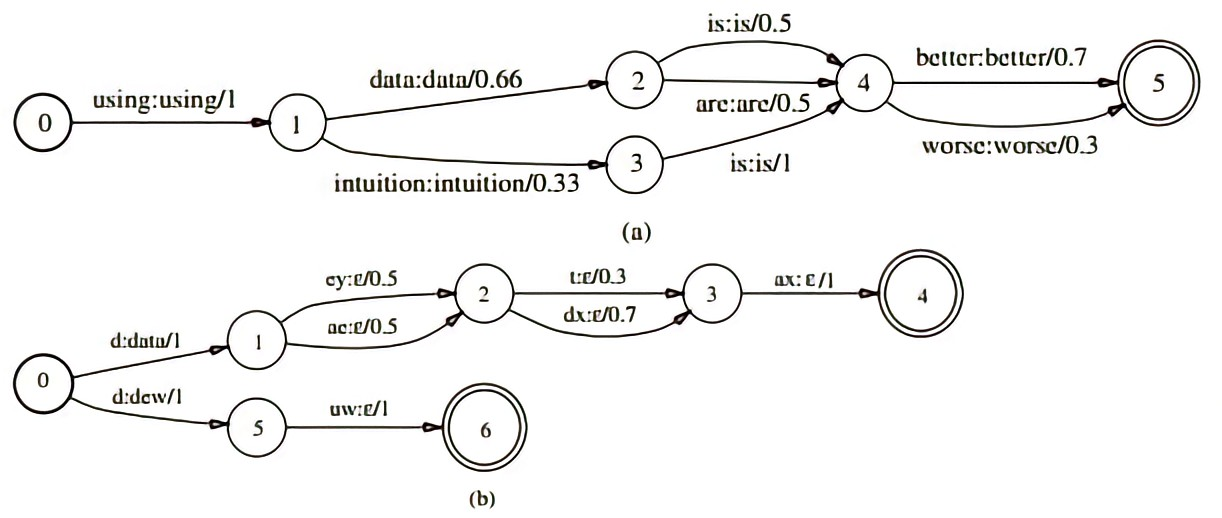
\includegraphics[width=3.5in, height=2in]{Fig3.jpg}}
\caption{Weighted Finite-state Transducer}
\label{fig:fstpic}
\end{figure}

\section{Experiment}
\label{sec:Experiment}
The main goal of our experiment is to decide which model could be better in terms of the performance by applying different approaches of training with different amount of data. The performance of ASR system is measured by WER on the acoustic models trained by different methods. In each experiment, each speech signal was parameterized using 13 MFCC. The analysis windows size was 23 ms with 10 ms overlap. We used 3-gram language model which is estimated from the training data transcription.

In our experiment, Hidden Markov Model-Gaussian Mixture (HMM-GMM) system is trained on top of MFCC features. Firstly, we trained a mono-phone system (mono) using the MFCC’s and Δ+ΔΔ features on the amount of different data. Then, we aligned the feature vectors to HMM states using utterances’ transcription. Finally, we retrain the triphone acoustic model on Linear Discriminant Analysis - Maximum Likelihood Linear Transform (LDA+MLLT) features and made speaker adaptive training (SAT). 

\subsection{Training Monophone Models (Mono)}
\label{sec:TrainingMonophoneModels}
A monophone model is an acoustic model and it does not include any contextual information about preceding or following phone. Additionally, it is used as a building block for the triphone models, which do make use of contextual information. In acoustic training steps, the parameters of the acoustic model are estimated, but the process can be better optimized by cycling through training and alignment phases. By aligning the audio to the reference transcript with the most current acoustic model, additional training algorithms can then use this output to improve or refine the parameters of the model. Therefore, each training step will be followed by an alignment step where the audio and text can be realigned.

\subsection{Training Tri-phone Models (Tri1)}
\label{sec:TrainingTri-phoneModels}
While monophone models simply represent the acoustic parameters of a single phoneme, phonemes will vary considerably depending on their particular context. However, in triphone models, a phoneme variant is represented in the context of two other (left and right) phonemes. At this point, there are 3 possible triphone models, but only a subset of those will actually occur in the data. Moreover, the unit must also occur multiple times in the data to gather sufficient statistics for the data. These triphones are grouped by a phonetic decision tree into a smaller amount of acoustically distinct units, thereby reducing the number of parameters and making the problem computationally feasible. Initially, in order to train a triphone system, we used the number of leaves, 200 and the total number of Gaussian across all states in our model, 1100 as our initial model size.

\subsection{Training Tri-phone Model with Δ+ΔΔ Features (Tri2)}
\label{sec:TrainingTri-phoneModelwithDelta}
Δ+ΔΔ training computes delta and double-delta features, or dynamic coefficients, to supplement the MFCC features. Δ+ΔΔ features are numerical estimates of the first and second order derivatives of the signal (features). Delta features are computed on the window of the original features; the delta-delta are then computed on the window of the delta-features.

\subsection{Training Tri-phone Model with LDA+MLLT Features (Tri2)}
\label{sec:TrainingTri-phoneModelwithLDA+MLLTFeatures}
LDA-MLLT means Linear Discriminant Analysis - Maximum Likelihood Linear Transform. It takes the feature vectors and builds HMM states, but with a reduced feature space for all data. The MLLT takes the reduced feature space from the LDA and then derives a unique transformation for each speaker. Therefore, MLLT is a step towards speaker normalization, as it minimizes differences among speakers.

\subsection{Speaker Adaptive Training (Tri3)}
\label{sec:SpeakerAdaptiveTraining}
We perform speaker adaptive training (SAT) for speaker and noise normalization by adapting to each specific speaker with a particular data transform. This results in more homogenous or standardized data, allowing the model to use its parameters on estimating variance due to the phoneme, as opposed to the speaker or recording environment.

\section{Evaluation}
\label{sec:Evaluation}
There are different methods to evaluate the quality of an ASR system. In this project, we used Word Error Rate (WER), a common metric of the performance of a speech recognition. The main difficulty of measuring performance lies in the fact that the recognized word sequence can have a different length from the reference word sequence. The WER is derived from the Levenshtein distance, but working at the word level ~\cite{wer}. This problem is solved by first aligning the recognized word sequence with the reference word sequence using dynamic string alignment. The formula for WER is as below, summing up the three types of errors (substitution, deletion, and insertion), over the length of the string as in (5).
\begin{equation}\tag{5}
 WER = 
  \frac{100*(S+I+D)}{N}
\end{equation}

Here, N is the number of words in the reference, S is the number of substitutions, I is the number of insertions and D is the number of deletions. A basic alignment example as follows:

Example 1:

\tab Reference:  \tab{\padauktext စဉ်းစား ပေး ပါ  **   ရှင်}

\tab Hypothesis:  \tab{\padauktext စဉ်းစား ပေး ပါ တယ် ရှင်}

\tab Eval:	\tab[4.4cm]I	
\begin{equation*}
 WER = 
  \frac{100*(0+1+0)}{4}
\end{equation*}

Example 2:

\tab Reference:  \tab{\padauktext ကား ရဲ့ အရှိန် ကို လျှော့ ပါ}

\tab Hypothesis:  \tab{\padauktext ကား ရဲ့ အရှိန် **  လျှော့ ပါ }

\tab Eval:	\tab[4cm]D	
\begin{equation*}
 WER = 
  \frac{100*(0+0+1)}{6}
\end{equation*}

\subsection{Evaluation on Training Data Size}
\label{sec:EvaluationTraining}
Four different data sizes – 2 hrs, 3 hrs, 5 hrs, and 6 hrs - are used for incremental training in our experiment. First of all, we analyzed the amount of data needed to train an mono-phone system (mono) and tri-phone systmes such as Tri1 (Δ+ΔΔ), Tri2 (LDA + MLLT) and Tri3 (SAT) by using number of leaves, 200 and total Gaussian number, 1100. Table~\ref{table:exp1Data}. shows the performance result of different acoustic training methods with incremental data. Based on this evaluation, we can claim that data size is a very important point in order to achieve enough recognition accuracy. 
\begin{table}[ht]
\caption{Word Error Rate \%  for Increasing Amount of Training Data} % title of Table
\centering % used for centering table
\setlength\tabcolsep{1.5pt} % default value: 6pt
\begin{tabular}{c c c c c} % centered columns (4 columns)
\hline %inserts double horizontal lines
Experiment & Mono & Tri1 & Tri2 & Tri3 \\  %[0.5ex] % inserts table
%heading
  &  & Δ+ΔΔ & (LDA+MLLT) & SAT  \\
\hline % inserts single horizontal line
1st Experiment (2hr) &  29.65 & 31.58 & 28.62 & 23.22\\
2nd Experiment (3hr) &  22.32 & 23.46 & 20.4 & 19.46\\
3rd Experiment (5hr) &  18.46 & 20.1 & 17.97 & 17.69\\
4th Experiment (6hr) &  \textbf{17.87}  & \textbf{19.54} & \textbf{16.35} & \textbf{16.44}\\[1ex] % [1ex] adds vertical space
\hline %inserts single line
\end{tabular}
\label{table:exp1Data} % is used to refer this table in the text
\end{table}

\subsection{Evaluation with N-gram Language Model}
\label{sec:EvaluationNGram}
Statistical language modeling has been used in different areas, consisting of speech recognition, optical character recognition, machine translation, and spelling correction, etc. Today, n-gram language models dominate as the technology of choice for current speech recognizer. Thus, in this task, the ASR accuracy is investigated based on different n-gram language models (LMs).  SRILM language modeling toolkit is applied to create the language model by using the default smoothing technique, good-tuning. The evaluation results of n-gram language models are depicted in Table~\ref{table:ngramData}.
\begin{table}[ht]
\caption{The WER \% of the ASR Performance with N-gram Language Model} % title of Table
\centering % used for centering table
\setlength\tabcolsep{1.5pt} % default value: 6pt
\begin{tabular}{c c c c c} % centered columns (4 columns)
\hline %inserts double horizontal lines
Language-Model & Mono & Tri1 & Tri2 & Tri3 \\  %[0.5ex] % inserts table
%heading
(n-gram)  &  & Δ+ΔΔ & (LDA+MLLT) & SAT  \\
\hline % inserts single horizontal line
0-gram &  58.35 & 61.62 & 58.55 & 57.97\\
1-gram &  47.68 & 50.84 & 47.09 & 48.09\\
2-gram &  20.69 & 22.33 & 18.79 & 19.33\\
\textbf{3-gram} &  \textbf{17.62}  & \textbf{19.54} & \textbf{16.35} & \textbf{16.44}\\
4-gram &  17.73 & 19.62 & 16.63 & 16.51\\
5-gram &  17.72 & 19.58 & 16.46 & 16.65\\[1ex] % [1ex] adds vertical space
\hline %inserts single line
\end{tabular}
\label{table:ngramData} % is used to refer this table in the text
\end{table}
From the table, it is found that the highest WERs are reached by using 0-gram LM (without language model). 3-gram based language model is the best and it has the lowest WERs among 0 to 5-gram. The lowest WERs, 17.62\% for Mono-phone, 19.54\% for Tri1 (Δ+ΔΔ), 16.35\% for Tri2 (LDA + MLLT) and 16.44\% for Tri3 (SAT) are obtained with 3-gram language model. As the result, it can be clearly proved that language model has an important role to improve ASR accuracy.

\subsection{Evaluation on Training with Different Model Size}
\label{sec:EvaluationDiffMS}
We re-trained the tri-phone model with two different transformation. Here, we used all amount of data available that is we used 6 hr audio data and 3-gram LM to train the acoustic models. Moreover, we evaluated the performance of the model depending on the model size. The performance obtained by training acoustic models on different model size can be seen in Table~\ref{table:diffMSData}.
\begin{table}[ht]
\caption{The WER \% of the ASR Performance using Different Model Size} % title of Table
\centering % used for centering table
\setlength\tabcolsep{1.5pt} % default value: 6pt
\begin{tabular}{c c c c c} % centered columns (4 columns)
\hline %inserts double horizontal lines
 Model Size & Model Size &  &  &   \\
No. of Leaves & Total No. of & Tri1 & Tri2 & Tri3 \\  %[0.5ex] % inserts table
%heading
  & Gaussian & Δ+ΔΔ & (LDA+MLLT) & SAT  \\
\hline % inserts single horizontal line
200 & 1100 & 19.54 & 16.35 & 16.44\\
200 & 3000 & 15.63 & 14.02 & 13.91\\
200 & 6000 & 15.82 & 14.38 & 13.54\\
500 & 1100 & 17.59 & 14.7 & 14.42\\
500 & 3000 & 12.9 & 11.71 & 11.02\\
500 & 6000 & 12.68 & 11.66 & 11.18\\
700 & 1100 & 17.36 & 14.65 & 14.25\\
700 & 3000 & 12.8 & 11.16 & 11.04\\
700 & 6000 & 12.17 & 10.82 & 10.4\\
1000 & 6000 & \textbf{11.95} & \textbf{10.63} & \textbf{10.21}\\[1ex] % [1ex] adds vertical space
\hline %inserts single line
\end{tabular}
\label{table:diffMSData} % is used to refer this table in the text
\end{table}

From this experiment, it can be observed that increasing the model size in average lead to better performance. Although each parameter alone improve the recognition, the most decisive parameter is the total number of Gaussian. Moreover, we can notice that LDA+MLLT upgrade almost 1\% the WER than transformation. LDA+MLLT works better than Δ+ΔΔ. 

\section{Conclusion}
\label{sec:conclusion}

ASR is a complex part of signal processing that has a lot of fields to study. In this project, different approaches to train and adapt acoustic models have been studied to be able to built an accurate automatic speech recognition system. The training part is defined as the most important step since it determines mainly the accuracy of our system. In our experiments, we observed a reduction of 11.78\% on Mono-phone, 12.04\% on Tri-phone (Δ+ΔΔ), 12.27\% on Tri-phone (LDA+MLLT) and 6.57\% on Tri-phone (SAT) in terms of word error rate during the incremental training. As more data obtainable, better results could be achieve. Moreover, the ASR performance is compared and evaluated based on different n-gram (0-gram to 5-gram) LMs and also on the different model size.  From our experiment results, 3-gram based language model and total number of Gaussian, 100 are the best for our system with the small amount of data. 

%\section*{Acknowledgment}

%We would like to thank %principals, teachers, SL trainers and students of School for the Deaf (Mandalay), Mary Chapman Chapman School for the Deaf Children (Yangon) and School for the Deaf, Tarmwe (Yangon), Myanmar Deaf Society and Literacy and Language Development for the Deaf for their kind contribution to our research. This research is partially supported by Ministry of Education, Department of Higher Education (Myanmar).

%%%%%%%%%%%%%%%%%%%%%%%%



%``Fig.~\ref{fig}'', even at the beginning of a sentence.

\begin{thebibliography}{00}

\bibitem{YKTG2P}Ye Kyaw Thu, et al. \quotes{Comparison of Grapheme-to-Phoneme Con-version Methods on a Myanmar Pronunciation Dictionary}. Proceedings of the 6th Workshop on South and Southeast Asian Natural Language Processing, pages 11-22, Osaka, Japan, December 11-17 2016.

\bibitem{howtostartKaldi}Yoav Ramon, \quotes{How to start with Kaldi and Speech Recognition}, https://towardsdatascience.co m/how-to-start-with-kaldi-and-speech-recognition-a9b7670ffff6, November 2018.

\bibitem{gmm}Virendra Chauhan, Shobhana Dwivedi, Pooja
Karale and Prof. S.M. Potdar, \quotes{Speech to Text Converter using Gaussian Mixture Model (GMM)}, Paper, International Research Journal of Engineering and Technology (IRJET), India, February 2016, pp. 160-164.

\bibitem{meKaldi}Emelie Kullmann, \quotes{Speech to Text for Swedish
using KALDI}, Master Thesis Book, KTH Royal Institute of Technology School of Engineering Sciences, Sweden, 2016.

\bibitem{stot}Madeline Briere, Automatic Speech Recognition
using the Kaldi Toolkit, madelinebriere.com, Duke
University, February 2018.

\bibitem{acmdl}Wolfgang Macherey, Discriminative Training and Acoustic Modeling for Automatic Speech Recognition, 2010.

\bibitem{srilm}A.Stolcke, \quotes{Srilm - An Extensible Language Modeling Toolkit}, pp. 901–904, 2002.

\bibitem{srec}P.K. Kurzekar, R.R. Deshmukh, V.B. Waghmare and P.P. Shrishrimal, \quotes{Continuous Speech Recog-nition System A Review}, Asian Journal of Computer Science and Information Technology, Vol. 4, No. 6, pp. 62-66, 2014.

\bibitem{wfst}Mohri, Pereira and Riley, Speech Recognition with Weighted Finite-State Transducers, in Springer Handbook on Speech Processing and Speech Communication, 2008.

\bibitem{wer}Shaghayegh Esmaeili, \quotes{Word Error Rate (WER) for Recognition of Natural Interactions}, Intelligent Natural Interaction Technology, April 2018.





\end{thebibliography}

\end{document}

